
\subsubsection{Modificando el \textit{dataset} para la red neuronal}\label{dataset-creation}

Una vez explicado el \textit{dataset} que se quiere conseguir junto con la motivación, se explicará en esta sección los pasos seguidos para conseguir dicho resultado. El \textit{dataset} que se tiene en este punto tiene tantas filas como viajes haya habido entre el 2014 y 2019. Por cada fila, se tienen dos atributos: \textit{from\_station\_id} y \textit{start\_time}. 
\newline

En este módulo se quiere modificar dicho \textit{dataset} para obtener otro que contenga los vectores que puedan ser usados como vectores de entrada en la red. Es decir, se quiere crear un \textit{dataset} que contenga en cada fila los intervalos y en cada columna los datos de dicho intervalo: \textit{hour}, \textit{day\_of\_week}, \textit{month} y \textit{quantity\_$j$}. Al finalizar todos los pasos de este módulo, los datos se guardarán en un archivo llamado \small{\verb|intervals.csv|} y se puede ver una muestra de estos datos en el Apéndice \ref{app:intervals_dataset}.
\newline

Primeramente, el código de este módulo, carga los datos del anterior módulo del archivo \acrshort{csv} \small{\verb|trips.csv|}:
\begin{minted}[fontsize=\footnotesize]{python}
import pandas as pd

# Read CSV as DataFrame an use datetime as index
df = pd.read_csv("/path/to/trips.csv", index="start_time")
\end{minted}

Una vez cargado el \small\verb|DataFrame| se han realizado los siguientes pasos:
\begin{enumerate}
    \item \underline{Agrupar los viajes por intervalos}: Este paso tiene como objetivo agrupar los viajes que se inician en cada una de las estaciones en intervalos. Se han estudiado diferentes tamaños de intervalos, como por ejemplo, intervalos de $15$ ó $30$ minutos, pero finalmente, se ha elegido 1 hora porque se reduce de forma considerable la cantidad de filas y sigue siendo un intervalo válido y no muy amplio.
    \newline
    
    Se han agrupado los distintos viajes en intervalos en función de la columna \textit{from\_station\_id} y \textit{start\_time}. Como ejemplo, suponga que en la variable \small{\verb|df|} se tiene el siguiente \small{\verb|DataFrame|}:

    \begin{table}[H]
    \footnotesize
    \centering
    \begin{tabular}{c|rr}
        \toprule
          \textit{start\_time} & \textit{from\_station\_id}  \\
        \midrule
        
        10:10 - 12/2/2018 & 48\\
        10:28 - 12/2/2018 & 15\\
        10:56 - 12/2/2018 & 15\\
        11:03 - 15/2/2018 & 15\\
        11:12 - 15/2/2018 & 48\\
        11:15 - 15/2/2018 & 15\\
        11:18 - 15/2/2018 & 15\\
        11:31 - 15/2/2018 & 15\\
        11:44 - 15/2/2018 & 48\\
        11:49 - 15/2/2018 & 15\\
        22:00 - 16/2/2018 & 15\\
        22:15 - 16/2/2018 & 48\\
        22:37 - 16/2/2018 & 193\\
        22:56 - 16/2/2018 & 48\\
        \bottomrule
        
    \end{tabular}
    \cprotect\caption{Ejemplo de \textit{dataset} guardado en \small{\verb|trips.csv|}}
    \label{tab:starttime_withsid}
    \end{table}
    
    El código usado para poder agrupar los viajes por intervalos y por estación ha sido el siguiente:
    
    \begin{minted}[fontsize=\footnotesize]{python}
INTERVAL = "1H"  # It could be also 15Min

df = df.groupby('from_station_id') \
       .resample(INTERVAL, on='start_time') \
       .size() \    # Resampling using the sum rule
       .to_frame()  # Converts it to DataFrame
    \end{minted}
    
    Tras ejecutar estas líneas de código y usando el ejemplo de la tabla \ref{tab:starttime_withsid} se puede observar que el resultado es el siguiente:
    
    \begin{table}[H]
    \footnotesize
    \centering
    \begin{tabular}{c|rr}
        \toprule
          \textit{start\_time} & \textit{from\_station\_id} & \textit{quantity}  \\
        \midrule
        
        10:00 - 12/2/2018 & 15 & 2\\
        10:00 - 12/2/2018 & 48 & 1\\
        10:00 - 12/2/2018 & 193 & 0\\
        11:00 - 15/2/2018 & 15 & 5\\
        11:00 - 15/2/2018 & 48 & 2\\
        11:00 - 15/2/2018 & 193 & 0\\
        22:00 - 16/2/2018 & 15 & 1\\
        22:00 - 16/2/2018 & 48 & 2\\
        22:00 - 16/2/2018 & 193 & 1\\
        \bottomrule
    \end{tabular}
    \cprotect\caption{Ejemplo del \textit{dataset} agrupados por estaciones y por intervalos.}
    \label{tab:justintervals}
    \end{table}
    
    

    \item \underline{Pivotar por intervalos}: Este paso tiene como objetivo agrupar todos los intervalos en uno solo, aumentando por tanto la cantidad de columnas y reduciendo la cantidad de filas. Es decir, se quiere tener que cada fila represente un intervalo y cada columna represente una estación. Usando el mismo ejemplo del paso anterior, el \small{\verb|DataFrame|} final quedaría de la siguiente manera:
    \begin{table}[H]
    \footnotesize
    \centering
    \begin{tabular}{c|rrr}
        \toprule
        \textit{start\_time} & \textit{quantity\_15} & \textit{quantity\_48} & \textit{quantity\_193}  \\
        \midrule
        10:00 - 12/2/2018 & 2 & 1 & 0 \\
        11:00 - 15/2/2018 & 5 & 2 & 0 \\
        22:00 - 16/2/2018 & 1 & 2 & 1 \\
        
        \bottomrule
    \end{tabular}
    \cprotect\caption{Ejemplo de \textit{dataset} que contiene los intervalos.}
    \label{tab:intervals_example}
    \end{table}
    
    Principalemente, el código usado para este paso hace uso de la función de \textit{pandas} denominada \small{\verb|pivot()|}:
    \begin{minted}[fontsize=\footnotesize]{python}
# Prepare the new columns names for each station
df["quantity_index"] = "quantity_" + \
                        df["from_station_id"].astype("str")

# We don't need from_station_id anymore
df = df.drop(columns=["from_station_id"])

# Make the pivot around quantity_index column and
# set the value of the column the same value as
# quantity from before saving quantity from
df = df.pivot(columns='quantity_index', values='quantity')

# If station any interval didn't have any trips for
# a station, then fill it with 0
return df.fillna(0)
    \end{minted}
    
    Si se compara la tabla \ref{tab:starttime_withsid} con la tabla \ref{tab:intervals_example} se puede ver que la cantidad de datos ha sido reducida considerablemente y se ha seleccionado solo la información necesaria que la red necesitará.
    \newline
    
    \item \underline{Obtener la variables de tiempo}: La columna \textit{start\_time} es una Serie con \textit{timestamps} y por lo tanto tiene información más de la necesaria (año, mes, día, hora, minuto, segundo...). La única información temporal que se necesita son un subconjunto de dichos valores. En concreto, los valores que se han creído ser útiles son: la hora, el día de la semana (no es lo mismo un lunes que un sábado) y el mes (no es lo mismo un mes de invierno que de verano). Estos son los valores más simples que se han usado pero eso no quita que se puedan usar otros datos que aportan más información como por ejemplo: día del mes, año o el minuto. 
    \newline
    
    Usando las variables de esta forma y no usando el \textit{timestamp} directamente a la red, el modelo puede aprender patrones en función de variables más simples como la hora, el día de la semana o el mes, y no con un número de 64 bits que apenas aporta información alguna puesto que la red lo tomaría como valores ascendentes sin ningún tipo de criterio.
    
    Para crear las nuevas columnas con los atributos que se han explicado anteriormente se han usado las siguientes líneas de código:
    \begin{minted}[fontsize=\footnotesize]{python}
# Index and start_time column is the same

df['hour'] = df.index.hour              # Number between 0-23
df['day_of_week'] = df.index.dayofweek  # Number between 0-6
df['month'] = df.index.month            # Number between 1-12
    \end{minted}
    
    Al final de este paso existirán por tanto las siguientes columnas para cada uno de los intervalos: \textit{start\_time}, \textit{hour}, \textit{day\_of\_week}, \textit{month} y una columna por cada estación. La columna \textit{start\_time} no se borra pues es la columna usada como índice y ayuda a la hora de entender la información con la que se trabaja. Pero no será usada por la red neuronal.
    \newline
    
    Usando el mismo ejemplo que los pasos anteriores, la tabla quedaría de la siguiente manera:
    \begin{table}[H]
    \footnotesize
    \centering
    \begin{tabular}{c|rrr|rrr}
        \toprule
        \textit{start\_time} & \textit{quantity\_15} & \textit{quantity\_48} & \textit{quantity\_193} & \textit{hour} & \textit{day\_of\_week} & \textit{month} \\
        \midrule
        10:00 - 12/2/2018 & 2 & 1 & 0 & 10 & 0 & 2 \\
        11:00 - 15/2/2018 & 5 & 2 & 0 & 11 & 3 & 2 \\
        22:00 - 16/2/2018 & 1 & 2 & 1 & 22 & 4 & 2 \\
        
        \bottomrule
    \end{tabular}
    \cprotect\caption{Ejemplo de \textit{dataset} final que será usada por la red neuronal.}
    \label{tab:intervals_example}
    \end{table}
    
    
    En este punto también se estudió la posibilidad de guardar la información de las variables temporales en forma de señal con valores entre los rangos $[-1, 1]$ usando seno y coseno \cite{reddit_time}. Esto permite que el modelo tenga acceso a la información temporal con valores continuos y no discretos como se puede ver en la figura \ref{fig:hour-stepvssignal} a continuación. Los resultados que se obtuvieron con ambas técnicas fueron similares, por lo que por simplicidad se dejo con valores discretos.
    
   \begin{figure}[H]
  \centering
  \subfloat[Hora con valores continuos de $-1$ a $1$]{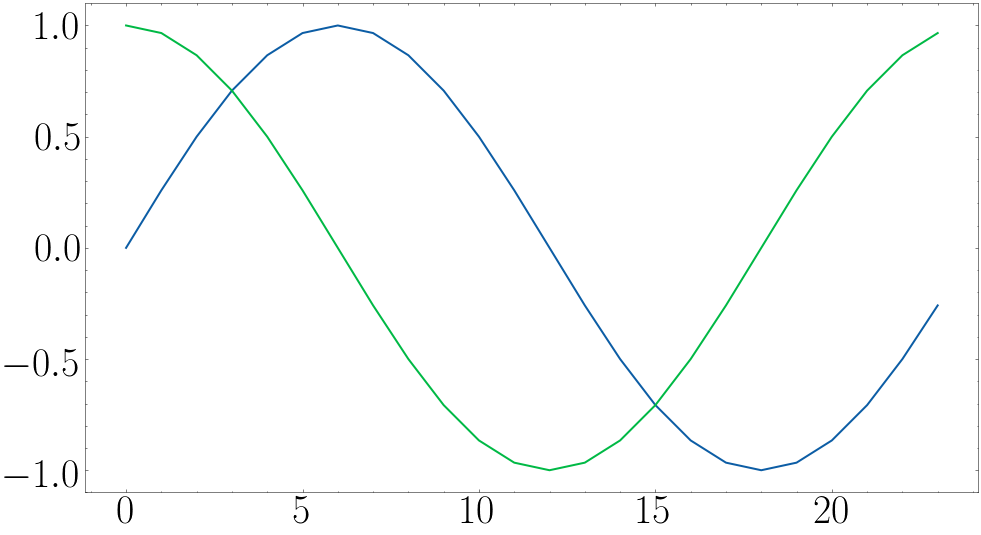
\includegraphics[width=0.4\textwidth]{images/solution/modules/hour_signal.png}\label{fig:f1}}
  \hfill
  \subfloat[Hora con valores discretos de $0$ a $23$]{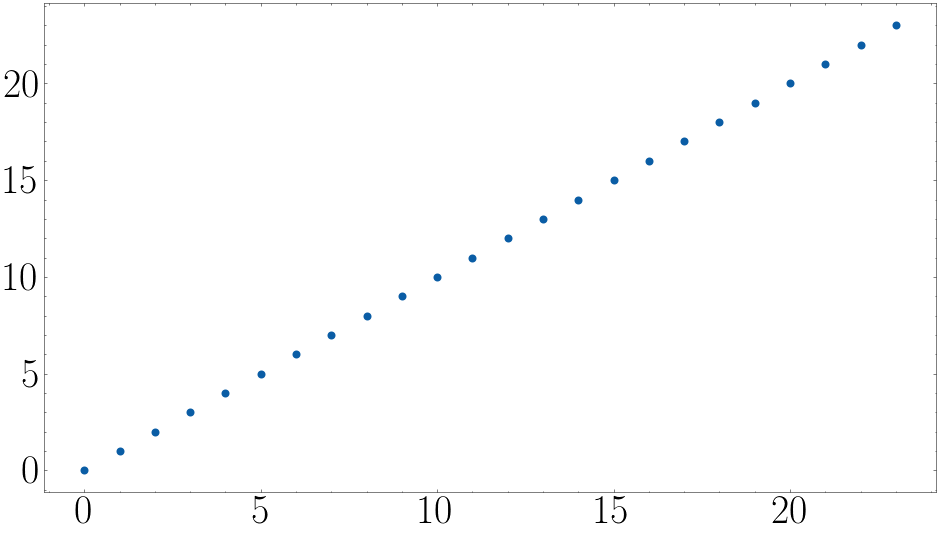
\includegraphics[width=0.4\textwidth]{images/solution/modules/hour_steps.png}\label{fig:f2}}
  \caption{Posibles formas de representar la variable \textit{hour}.}
  \label{fig:hour-stepvssignal}
\end{figure}
    
\end{enumerate}


El \small{\verb|DataFrame|} obtenido por este módulo se guarda en un fichero \acrshort{csv} llamado \small{\verb|intervals.csv|} que será usado por los siguientes módulos cuyo contenido tendrá una estructura similar a la que se muestra en la tabla \ref{tab:intervals_example}.

\begin{minted}[fontsize=\footnotesize]{python}
# Save df in a CSV file
df.to_csv("path/to/intervals.csv")
\end{minted}